% rotate-reverse.tex

\documentclass[tikz]{standalone}
\usetikzlibrary{shapes.multipart, positioning}

\begin{document}
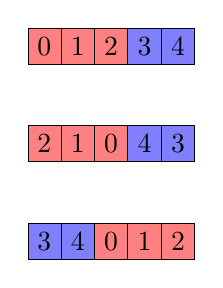
\begin{tikzpicture}[array/.style = {
    rectangle split, rectangle split parts = #1, 
    rectangle split horizontal, 
    rectangle split part fill = {red!50, red!50, red!50, blue!50, blue!50},
    draw, anchor = center, minimum width = 0.60cm}]
  \node (a) [array = 5] {0\nodepart{two}1\nodepart{three}2\nodepart{four}3\nodepart{five}4};

  \node (reverse) [array = 5, below = of a.center]
    {2\nodepart{two}1\nodepart{three}0\nodepart{four}4\nodepart{five}3};

  \node [array = 5, below = of reverse.center,
    rectangle split part fill = {blue!50, blue!50, red!50}] 
    {3\nodepart{two}4\nodepart{three}0\nodepart{four}1\nodepart{five}2};
\end{tikzpicture}
\end{document}